% !TEX root = fce.tex
% -----------------------------------------------------------------
% Filename  :	task5.tex
% Author    :	Meyer zum Felde, Püttjer, Hoppe
% Date		:	18.03.2017
% -----------------------------------------------------------------

\subsection{Branch Prediciton}
\label{sec:branchPrediction}

The task was to implement a branch prediction unit in three ways:

\begin{itemize}
\item ``Static branch prediction''
\item ``Dynamic branch prediction using a branch history table (BHT)''
\item ``dynamic branch prediction using a branch target buffer (BTB)''
\end{itemize}

\subsection{Static Branch Prediciton}
\label{sec:staticBranchPrediction}

For our static branch prediction we needed perform the check if a branch will be taken in the ID phase. The comfortable restriction that was given was the fact that we only need to handle the commands BNE and BEQ since they were the ones used for testing programs like isort\_pipe. In fact no other assembler file given was using other branch commands. Therefore our branch predicition only needed to handle a comparison check of two given registers. This was implemented using the following technique. 

We inserted a new signal called branchIdPhase. This signal was set to 1 whenever a BEQ or BNE command was detected in the ID phase and simultaneously not in MA or EX phase. We wanted it to be set to '1' in order to mark the arrival of a new branch command. Simultenously our signal predictionError receives the input to perform static jumping if our StaticBranchAlwaysTaken signal is set to '1' and the branch condition is not met. In other words if we assume a branch is always taken and the condition to take a branched step is not given our predictionError signal is set to '1'. Whenever we have a predictionError we decide to take another path than the one that was predicted.

\lstinputlisting[caption={BranchCheckMovedToIDPhase}]{appendix/task5_change1_frontAdded.txt}

The impact of our code was to let the system assume a certain strategy like always ``always assume to take a branch'' and performing stalling whenever the prediction was not right. We needed to test whether this strategy was running as well as the possibility to switch the strategy at any time since the logic would be used in the dynamic branching also.


\subsection{Dynamic Branch Prediction Using a BHT}
\label{sec:dynamicBranchPredictionUsingBHT}

In the beginning understanding of the functionality of a BHT needed to be gained. This was done by using the preinstalled feature from the MARS simulator. 
Which can be seen in figure \ref{fig5-1} on page \pageref{fig5-1}.

\begin{figure}
	\centering
  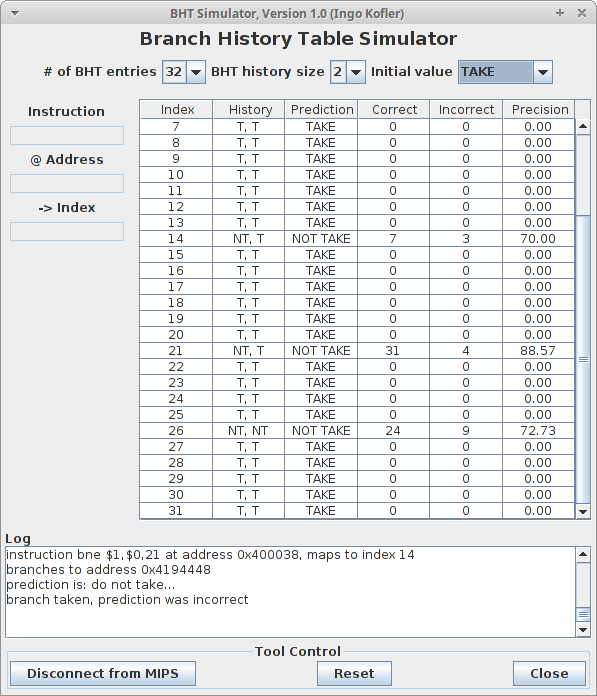
\includegraphics[width=1\textwidth, keepaspectratio]{pictures/task5_BHT_sim_1}
	\caption{Screenshot of BHT Simulation in MARS using isort\_pipe from lecture}
	\label{fig5-1}
\end{figure}

The BHT basically uses a slot for each branch command and remembers the last one or two jumping behaviours. According to the history the next jump should be taken in order to guess as many tries as possible correctly. Our problem is that whenenver we guess our branch jump behaviour wrong, we lose clock cycles. Therefore we want a prediction rate as high as possible. 

The interesting thing is if we compare values for changed input like Intitial state either ``TAKE'' or ``NOT TAKE'' and History size is either 2 or only 1 entry we can see following behaviour in table \ref{tab5-1} on page \pageref{tab5-1}. Additional screenshots of results can be seen in the appendix.

\begin{table}[h]
\resizebox{1\textwidth}{!}{\begin{minipage}{\textwidth}
\begin{tabular}{ l l l l l }
 \hline
 BHT Settings & 1BNE Precision & 2BNE Precision & BEQ Precision\\ \hline

 BHT with History 1 Initial TAKE & 80\% & 88.57\% & 72.73\% \\
 BHT with History 2 Initial TAKE & 70\% & 88.57\% & 72.73\% \\
 BHT with History 1 Initial NOT TAKE & 90\% & 91.43\% & 69.70\% \\
 BHT with History 2 Initial NOT TAKE & 90\% & 94.29\% &75.76\% \\
	\hline
\end{tabular}
\caption[Table caption text]{of successful prediction using BHT in isort\_pipe}
\label{tab5-1}
\end{minipage} }
\end{table}


\subsection{Dynamic Branch Prediction using BTB}

\subsection{Lessons Learned}
Wnile doing the work of this section another problem occured. Since we were three people using three different OS one of our computers was not able to accept a correct Eclipse Sigasi Certificate on an emulated Linux machine running on a physical Macbook. The workaround at hand was to implement the code on the Mac OS, upload the code using github and pulling the modified  state on the virtual Linux machine. Tests were run in the virtual box but the coding had to be done on the physical OS. This was a bit of a slow down factor since each change of code caused a push and pull action for this team member. We recommend again to use the same OS on all systems and the same Development Software on all machines. For our case we needed some workarounds.
